\documentclass{article}
\pagestyle{empty}
\usepackage{tikz}
\usetikzlibrary{arrows.meta,decorations.pathreplacing}
\definecolor{diagOrange}{RGB}{240,105,26}
\definecolor{boxFill}{RGB}{239,239,239}
\definecolor{boxStroke}{RGB}{154,154,154}
\definecolor{inkGray}{RGB}{51,51,51}
\begin{document}
\noindent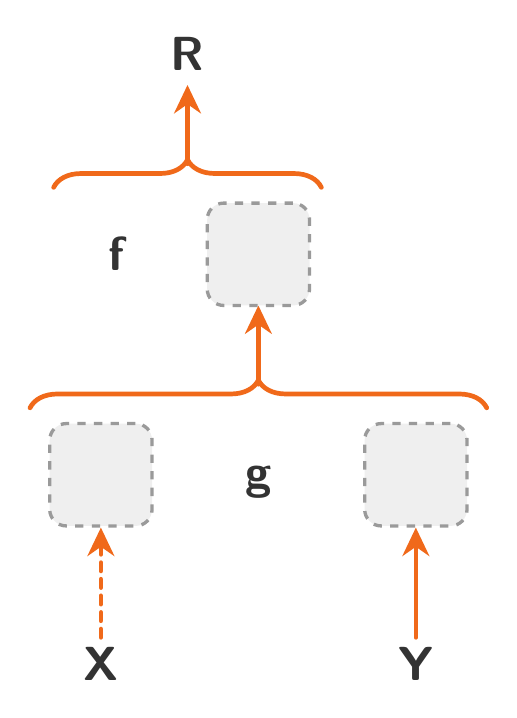
\begin{tikzpicture}[
  >={Stealth[length=3.6mm,width=3.4mm]}, line join=round,
  slot/.style={draw=boxStroke, dashed, line width=1.2pt, rounded corners=6pt,
               fill=boxFill, minimum size=1.3cm},
  flow/.style={diagOrange, line width=1.7pt, line cap=round, ->},
  flowdash/.style={diagOrange, line width=1.7pt, line cap=round, dashed, ->},
  brace/.style={diagOrange, line width=1.7pt, line cap=round,
                decorate, decoration={brace, amplitude=10pt}},
  lbl/.style={inkGray, font=\sffamily\bfseries\LARGE},
]
  \node[lbl] (X) at (1.5,0.2) {X};
  \node[lbl] (Y) at (5.5,0.2) {Y};
  \node[slot] (gL) at (1.5,2.6) {};
  \node[slot] (gR) at (5.5,2.6) {};
  \draw[flowdash] (X) -- (gL);
  \draw[flow]     (Y) -- (gR);
  \draw[brace] (0.6,3.45) -- (6.4,3.45);
  \node[lbl] at (3.5,2.5) {g};
  \draw[flow] (3.5,3.75) -- (3.5,4.75);
  \node[slot] (fBox) at (3.5,5.4) {};
  \draw[brace] (0.9,6.25) -- (4.3,6.25);
  \node[lbl] at (1.7,5.4) {f};
  \draw[flow] (2.6,6.55) -- (2.6,7.55);
  \node[lbl] (R) at (2.6,7.95) {R};
\end{tikzpicture}
\end{document}
